\documentclass[12pt,a4paper]{article}

%\pdfoutput=1

\usepackage[utf8]{inputenc}
\usepackage[T1]{fontenc}
\usepackage[english]{babel}
\usepackage{amsmath}
\usepackage{lmodern}
\usepackage{units}
\usepackage{siunitx}
\usepackage{icomma}
\usepackage{graphicx}
\usepackage{caption}
\usepackage{subcaption}
\usepackage{color}
\usepackage{pgf}
\DeclareMathOperator{\acosh}{arccosh}
\newcommand{\N}{\ensuremath{\mathbbm{N}}}
\newcommand{\Z}{\ensuremath{\mathbbm{Z}}}
\newcommand{\Q}{\ensuremath{\mathbbm{Q}}}
\newcommand{\R}{\ensuremath{\mathbbm{R}}}
\newcommand{\C}{\ensuremath{\mathbbm{C}}}
\newcommand{\rd}{\ensuremath{\mathrm{d}}}
\newcommand{\id}{\ensuremath{\,\rd}}
\usepackage{hyperref}
%\usepackage{a4wide} % puts the page numbering further down the page.
\usepackage{pdfpages}
\usepackage{epstopdf}
\DeclareGraphicsExtensions{.eps}

\title{HFSS part 2: Chebyshev transformer}
\author{Marcus Malmquist, marmalm, 941022}
\date{\today}

\begin{document}
\maketitle

\section{Task 1}\label{sec:1}
This part involved designing a Chebyshev transformer (with a center frequency of $\SI{6}{\giga\hertz}$ for a waveguide with dimensions $a=\SI{80}{\milli\metre}$ and $b=\SI{10}{\milli\metre}$) with some predefined properties depending on assigned design id. For me the design id was 6 which means that I used the filter properties in Table~\ref{tab:filter_prop}

\begin{table}
  \centering
  \caption{Design constraints of the Chebyshev transformer.}
  \begin{tabular}{|c|c|c|c|}\hline
    Design ID & $\frac{Z_0}{Z_L}$ & Fractional & $\Gamma_m$ \\
     & & bandwidth & \\ \hline
    6 & 3.4 & 1 & 0.07 \\ \hline
  \end{tabular}
  \label{tab:filter_prop}
\end{table}
\noindent The fractional bandwidth presented in Table~\ref{tab:filter_prop} can be used to calculate $\theta_m$ using (\ref{eq:bw_frac})
\begin{equation}
  1=\dfrac{\Delta f}{f_0}=2-\dfrac{4\theta_m}{\pi}\Leftrightarrow \theta_m=\dfrac{\pi}{4}
  \label{eq:bw_frac}
\end{equation}
When $\theta_m$ is known the number of sections needed can be calculated using (\ref{eq:N})
\begin{equation}
  \cos^{-1}{\theta_m}=\cosh\Big[\dfrac{1}{N}\acosh\Big(\dfrac{1}{\Gamma_m}\Big|\dfrac{Z_L-Z_0}{Z_L+Z_0}\Big|\Big)\Big] 
  \label{eq:N}
\end{equation}

Since the resulting value of $N$ from (\ref{eq:N}) is not an integer it has to be rounded off and used to calculate a new value of $\theta_m$. The result is $N=3$ and $\theta_m\approx 0.808$.

When the number of sections is known what remains is to calculate the reflection coefficien $\Gamma$ in each interface and from there calculate what wave impedances are needed in the sections. By matching the total reflection coefficient and its components to the Chebyshev polynom (type I) corresponging to the number of sections using (\ref{eq:Gamma})
\begin{equation}
  \Gamma(\theta)=2e^{-j3\theta}\sum_n\big(\Gamma_n\cos(N-2n)\theta\big)=-\Gamma_me^{-j3\theta}T_N\Big(\frac{\cos\theta}{\cos\theta_m}\Big)
  \label{eq:Gamma}
\end{equation}
In this case we have $N=3$ and $T_3(x)=4x^3-3x$ so the reflection coefficients can be gotten by equating cosine terms as seen in (\ref{eq:Gamma_res})
\begin{subequations}
  \begin{align}
    \Gamma_0=\Gamma_3&=-\frac{\Gamma_m}{2\cos^{2}\theta_m}, \label{eq:Gamma_res1} \\
    \Gamma_1=\Gamma_2&=-\frac{3}{2}\Gamma_m\Big(\frac{1}{\cos^{3}\theta_m}-\frac{1}{\cos\theta_m}\Big)\label{eq:Gamma_res2}
  \end{align}
  \label{eq:Gamma_res}
\end{subequations}
then the characteristic impedances can be acquired from (\ref{eq:imp})
\begin{equation}
  Z_{i+1}=Z_i\frac{1+\Gamma_i}{1-\Gamma_i}
  \label{eq:imp}
\end{equation}

We now encounter a potential problem because (\ref{eq:Gamma_res}) and (\ref{eq:imp}) can be used to calculate the ratio between $Z_{L}$ and $Z_{0}$, but this can also be calculated since the ratio $\frac{Z_{0}}{Z_{L}}$ was given as a design property. As it truns out those expressions do not match so this problem has no solution. Instead we have to find the solution that have properties that are as close to those in Table~\ref{tab:filter_prop} as possible. This will be done by minimizing (\ref{eq:tar_fun}) with the condition that (\ref{eq:condition1}) and (\ref{eq:condition2}) must be fulfilled. (\ref{eq:condition1}) comes from the fact that $\Gamma_{m}$ must be the same in (\ref{eq:Gamma_res1}) and (\ref{eq:Gamma_res2}) while (\ref{eq:condition2}) comes from the fact that recursive use of (\ref{eq:imp}) must yield the same ratio between $Z_{L}$ and $Z_{0}$ as the ratio given as a design property.
\begin{subequations}
  \begin{align}
    f(\theta^{'}_{m},\Gamma^{'}_{0}, \Gamma^{'}_{1})&=\Big(\frac{|\theta^{'}_{m}-\theta_{m}|}{\theta_{m}}\Big)^{2}+\Big(\frac{|\Gamma^{'}_{0}-\Gamma_{0}|}{\Gamma_{0}}\Big)^{2}+\Big(\frac{|\Gamma^{'}_{1}-\Gamma_{1}|}{\Gamma_{1}}\Big)^{2}, \label{eq:tar_fun} \\
    \Gamma^{'}_{0}&=\frac{\Gamma^{'}_{1}}{3\sin^3\theta_{m}}, \label{eq:condition1} \\
    \frac{Z_L}{Z_0}&=\Big(\frac{1+\Gamma^{'}_0}{1-\Gamma^{'}_0}\Big)^{2}\Big(\frac{1+\Gamma^{'}_1}{1-\Gamma^{'}_1}\Big)^{2}, \label{eq:condition2}
  \end{align}
  \label{eq:optimize}
\end{subequations}
The result from this optimization problem was $\min f(\theta^{'}_{m},\Gamma^{'}_{0}, \Gamma^{'}_{1})=0.31453276$ after the final iteration (and $0.3959806$ after one iteration) and the final values can be seen in Table~\ref{tab:final_val} and the theoretical $\text{S}_{11}$ plot can be seen in Figure~\ref{fig:theoretical}
\begin{table}
  \centering
  \caption{Final transformer properties after optimization.}
  \begin{tabular}{|c|c|}\hline
    Property & Value \\ \hline
    $\frac{Z_{0}}{Z_{L}}$ & 3.4 \\ \hline
    $\Gamma_{m}$ & 0.077 \\ \hline
    $\frac{\Delta f}{f_{0}}$ & 0.969 \\ \hline
    $N$ & 3 \\ \hline
    $\theta_{m}$ & 0.810 \\ \hline
  \end{tabular}
  \label{tab:final_val}
\end{table}
\begin{figure}
  \centering
  \noindent\makebox[\textwidth]{\scalebox{0.9}{%% Creator: Matplotlib, PGF backend
%%
%% To include the figure in your LaTeX document, write
%%   \input{<filename>.pgf}
%%
%% Make sure the required packages are loaded in your preamble
%%   \usepackage{pgf}
%%
%% Figures using additional raster images can only be included by \input if
%% they are in the same directory as the main LaTeX file. For loading figures
%% from other directories you can use the `import` package
%%   \usepackage{import}
%% and then include the figures with
%%   \import{<path to file>}{<filename>.pgf}
%%
%% Matplotlib used the following preamble
%%   \usepackage{fontspec}
%%   \setmainfont{DejaVu Serif}
%%   \setsansfont{DejaVu Sans}
%%   \setmonofont{DejaVu Sans Mono}
%%
\begingroup%
\makeatletter%
\begin{pgfpicture}%
\pgfpathrectangle{\pgfpointorigin}{\pgfqpoint{8.000000in}{6.000000in}}%
\pgfusepath{use as bounding box, clip}%
\begin{pgfscope}%
\pgfsetbuttcap%
\pgfsetmiterjoin%
\definecolor{currentfill}{rgb}{1.000000,1.000000,1.000000}%
\pgfsetfillcolor{currentfill}%
\pgfsetlinewidth{0.000000pt}%
\definecolor{currentstroke}{rgb}{1.000000,1.000000,1.000000}%
\pgfsetstrokecolor{currentstroke}%
\pgfsetdash{}{0pt}%
\pgfpathmoveto{\pgfqpoint{0.000000in}{0.000000in}}%
\pgfpathlineto{\pgfqpoint{8.000000in}{0.000000in}}%
\pgfpathlineto{\pgfqpoint{8.000000in}{6.000000in}}%
\pgfpathlineto{\pgfqpoint{0.000000in}{6.000000in}}%
\pgfpathclose%
\pgfusepath{fill}%
\end{pgfscope}%
\begin{pgfscope}%
\pgfsetbuttcap%
\pgfsetmiterjoin%
\definecolor{currentfill}{rgb}{1.000000,1.000000,1.000000}%
\pgfsetfillcolor{currentfill}%
\pgfsetlinewidth{0.000000pt}%
\definecolor{currentstroke}{rgb}{0.000000,0.000000,0.000000}%
\pgfsetstrokecolor{currentstroke}%
\pgfsetstrokeopacity{0.000000}%
\pgfsetdash{}{0pt}%
\pgfpathmoveto{\pgfqpoint{1.000000in}{0.600000in}}%
\pgfpathlineto{\pgfqpoint{7.200000in}{0.600000in}}%
\pgfpathlineto{\pgfqpoint{7.200000in}{5.400000in}}%
\pgfpathlineto{\pgfqpoint{1.000000in}{5.400000in}}%
\pgfpathclose%
\pgfusepath{fill}%
\end{pgfscope}%
\begin{pgfscope}%
\pgfpathrectangle{\pgfqpoint{1.000000in}{0.600000in}}{\pgfqpoint{6.200000in}{4.800000in}} %
\pgfusepath{clip}%
\pgfsetrectcap%
\pgfsetroundjoin%
\pgfsetlinewidth{1.003750pt}%
\definecolor{currentstroke}{rgb}{0.000000,0.000000,0.000000}%
\pgfsetstrokecolor{currentstroke}%
\pgfsetdash{}{0pt}%
\pgfpathmoveto{\pgfqpoint{1.000000in}{4.758892in}}%
\pgfpathlineto{\pgfqpoint{1.024825in}{4.757540in}}%
\pgfpathlineto{\pgfqpoint{1.049650in}{4.753486in}}%
\pgfpathlineto{\pgfqpoint{1.074474in}{4.746735in}}%
\pgfpathlineto{\pgfqpoint{1.099299in}{4.737295in}}%
\pgfpathlineto{\pgfqpoint{1.124124in}{4.725179in}}%
\pgfpathlineto{\pgfqpoint{1.148949in}{4.710400in}}%
\pgfpathlineto{\pgfqpoint{1.173774in}{4.692977in}}%
\pgfpathlineto{\pgfqpoint{1.198599in}{4.672932in}}%
\pgfpathlineto{\pgfqpoint{1.223423in}{4.650290in}}%
\pgfpathlineto{\pgfqpoint{1.248248in}{4.625078in}}%
\pgfpathlineto{\pgfqpoint{1.279279in}{4.589996in}}%
\pgfpathlineto{\pgfqpoint{1.310310in}{4.551016in}}%
\pgfpathlineto{\pgfqpoint{1.341341in}{4.508212in}}%
\pgfpathlineto{\pgfqpoint{1.372372in}{4.461666in}}%
\pgfpathlineto{\pgfqpoint{1.403403in}{4.411468in}}%
\pgfpathlineto{\pgfqpoint{1.440641in}{4.346546in}}%
\pgfpathlineto{\pgfqpoint{1.477878in}{4.276682in}}%
\pgfpathlineto{\pgfqpoint{1.515115in}{4.202068in}}%
\pgfpathlineto{\pgfqpoint{1.552352in}{4.122911in}}%
\pgfpathlineto{\pgfqpoint{1.595796in}{4.025108in}}%
\pgfpathlineto{\pgfqpoint{1.639239in}{3.921780in}}%
\pgfpathlineto{\pgfqpoint{1.688889in}{3.797418in}}%
\pgfpathlineto{\pgfqpoint{1.738539in}{3.666943in}}%
\pgfpathlineto{\pgfqpoint{1.794394in}{3.513635in}}%
\pgfpathlineto{\pgfqpoint{1.856456in}{3.336283in}}%
\pgfpathlineto{\pgfqpoint{1.924725in}{3.134204in}}%
\pgfpathlineto{\pgfqpoint{2.005405in}{2.888341in}}%
\pgfpathlineto{\pgfqpoint{2.129530in}{2.501910in}}%
\pgfpathlineto{\pgfqpoint{2.284685in}{2.020024in}}%
\pgfpathlineto{\pgfqpoint{2.365365in}{1.776420in}}%
\pgfpathlineto{\pgfqpoint{2.433634in}{1.576801in}}%
\pgfpathlineto{\pgfqpoint{2.495696in}{1.401943in}}%
\pgfpathlineto{\pgfqpoint{2.551552in}{1.250923in}}%
\pgfpathlineto{\pgfqpoint{2.601201in}{1.122382in}}%
\pgfpathlineto{\pgfqpoint{2.650851in}{0.999726in}}%
\pgfpathlineto{\pgfqpoint{2.700501in}{0.883416in}}%
\pgfpathlineto{\pgfqpoint{2.743944in}{0.787182in}}%
\pgfpathlineto{\pgfqpoint{2.787387in}{0.696381in}}%
\pgfpathlineto{\pgfqpoint{2.830831in}{0.611240in}}%
\pgfpathlineto{\pgfqpoint{2.837037in}{0.600448in}}%
\pgfpathlineto{\pgfqpoint{2.874274in}{0.668040in}}%
\pgfpathlineto{\pgfqpoint{2.911512in}{0.731202in}}%
\pgfpathlineto{\pgfqpoint{2.948749in}{0.789841in}}%
\pgfpathlineto{\pgfqpoint{2.985986in}{0.843886in}}%
\pgfpathlineto{\pgfqpoint{3.017017in}{0.885369in}}%
\pgfpathlineto{\pgfqpoint{3.048048in}{0.923595in}}%
\pgfpathlineto{\pgfqpoint{3.079079in}{0.958546in}}%
\pgfpathlineto{\pgfqpoint{3.110110in}{0.990212in}}%
\pgfpathlineto{\pgfqpoint{3.141141in}{1.018593in}}%
\pgfpathlineto{\pgfqpoint{3.172172in}{1.043695in}}%
\pgfpathlineto{\pgfqpoint{3.203203in}{1.065533in}}%
\pgfpathlineto{\pgfqpoint{3.234234in}{1.084127in}}%
\pgfpathlineto{\pgfqpoint{3.259059in}{1.096688in}}%
\pgfpathlineto{\pgfqpoint{3.283884in}{1.107211in}}%
\pgfpathlineto{\pgfqpoint{3.308709in}{1.115719in}}%
\pgfpathlineto{\pgfqpoint{3.333534in}{1.122237in}}%
\pgfpathlineto{\pgfqpoint{3.358358in}{1.126792in}}%
\pgfpathlineto{\pgfqpoint{3.383183in}{1.129417in}}%
\pgfpathlineto{\pgfqpoint{3.408008in}{1.130144in}}%
\pgfpathlineto{\pgfqpoint{3.432833in}{1.129010in}}%
\pgfpathlineto{\pgfqpoint{3.457658in}{1.126056in}}%
\pgfpathlineto{\pgfqpoint{3.488689in}{1.119869in}}%
\pgfpathlineto{\pgfqpoint{3.519720in}{1.110992in}}%
\pgfpathlineto{\pgfqpoint{3.550751in}{1.099521in}}%
\pgfpathlineto{\pgfqpoint{3.581782in}{1.085558in}}%
\pgfpathlineto{\pgfqpoint{3.612813in}{1.069209in}}%
\pgfpathlineto{\pgfqpoint{3.643844in}{1.050588in}}%
\pgfpathlineto{\pgfqpoint{3.681081in}{1.025410in}}%
\pgfpathlineto{\pgfqpoint{3.718318in}{0.997344in}}%
\pgfpathlineto{\pgfqpoint{3.755556in}{0.966613in}}%
\pgfpathlineto{\pgfqpoint{3.798999in}{0.927705in}}%
\pgfpathlineto{\pgfqpoint{3.842442in}{0.885871in}}%
\pgfpathlineto{\pgfqpoint{3.892092in}{0.834988in}}%
\pgfpathlineto{\pgfqpoint{3.947948in}{0.774559in}}%
\pgfpathlineto{\pgfqpoint{4.016216in}{0.697383in}}%
\pgfpathlineto{\pgfqpoint{4.096897in}{0.603626in}}%
\pgfpathlineto{\pgfqpoint{4.103103in}{0.603626in}}%
\pgfpathlineto{\pgfqpoint{4.221021in}{0.739844in}}%
\pgfpathlineto{\pgfqpoint{4.289289in}{0.815179in}}%
\pgfpathlineto{\pgfqpoint{4.345145in}{0.873436in}}%
\pgfpathlineto{\pgfqpoint{4.394795in}{0.921898in}}%
\pgfpathlineto{\pgfqpoint{4.438238in}{0.961249in}}%
\pgfpathlineto{\pgfqpoint{4.481682in}{0.997344in}}%
\pgfpathlineto{\pgfqpoint{4.518919in}{1.025410in}}%
\pgfpathlineto{\pgfqpoint{4.556156in}{1.050588in}}%
\pgfpathlineto{\pgfqpoint{4.587187in}{1.069209in}}%
\pgfpathlineto{\pgfqpoint{4.618218in}{1.085558in}}%
\pgfpathlineto{\pgfqpoint{4.649249in}{1.099521in}}%
\pgfpathlineto{\pgfqpoint{4.680280in}{1.110992in}}%
\pgfpathlineto{\pgfqpoint{4.711311in}{1.119869in}}%
\pgfpathlineto{\pgfqpoint{4.742342in}{1.126056in}}%
\pgfpathlineto{\pgfqpoint{4.767167in}{1.129010in}}%
\pgfpathlineto{\pgfqpoint{4.791992in}{1.130144in}}%
\pgfpathlineto{\pgfqpoint{4.816817in}{1.129417in}}%
\pgfpathlineto{\pgfqpoint{4.841642in}{1.126792in}}%
\pgfpathlineto{\pgfqpoint{4.866466in}{1.122237in}}%
\pgfpathlineto{\pgfqpoint{4.891291in}{1.115719in}}%
\pgfpathlineto{\pgfqpoint{4.916116in}{1.107211in}}%
\pgfpathlineto{\pgfqpoint{4.940941in}{1.096688in}}%
\pgfpathlineto{\pgfqpoint{4.965766in}{1.084127in}}%
\pgfpathlineto{\pgfqpoint{4.990591in}{1.069510in}}%
\pgfpathlineto{\pgfqpoint{5.021622in}{1.048323in}}%
\pgfpathlineto{\pgfqpoint{5.052653in}{1.023876in}}%
\pgfpathlineto{\pgfqpoint{5.083684in}{0.996151in}}%
\pgfpathlineto{\pgfqpoint{5.114715in}{0.965142in}}%
\pgfpathlineto{\pgfqpoint{5.145746in}{0.930847in}}%
\pgfpathlineto{\pgfqpoint{5.176777in}{0.893275in}}%
\pgfpathlineto{\pgfqpoint{5.207808in}{0.852442in}}%
\pgfpathlineto{\pgfqpoint{5.238839in}{0.808370in}}%
\pgfpathlineto{\pgfqpoint{5.276076in}{0.751255in}}%
\pgfpathlineto{\pgfqpoint{5.313313in}{0.689591in}}%
\pgfpathlineto{\pgfqpoint{5.350551in}{0.623465in}}%
\pgfpathlineto{\pgfqpoint{5.362963in}{0.600448in}}%
\pgfpathlineto{\pgfqpoint{5.381582in}{0.634977in}}%
\pgfpathlineto{\pgfqpoint{5.418819in}{0.709011in}}%
\pgfpathlineto{\pgfqpoint{5.462262in}{0.800602in}}%
\pgfpathlineto{\pgfqpoint{5.505706in}{0.897593in}}%
\pgfpathlineto{\pgfqpoint{5.549149in}{0.999726in}}%
\pgfpathlineto{\pgfqpoint{5.598799in}{1.122382in}}%
\pgfpathlineto{\pgfqpoint{5.648448in}{1.250923in}}%
\pgfpathlineto{\pgfqpoint{5.704304in}{1.401943in}}%
\pgfpathlineto{\pgfqpoint{5.766366in}{1.576801in}}%
\pgfpathlineto{\pgfqpoint{5.834635in}{1.776420in}}%
\pgfpathlineto{\pgfqpoint{5.915315in}{2.020024in}}%
\pgfpathlineto{\pgfqpoint{6.020821in}{2.346694in}}%
\pgfpathlineto{\pgfqpoint{6.238038in}{3.021512in}}%
\pgfpathlineto{\pgfqpoint{6.318719in}{3.263560in}}%
\pgfpathlineto{\pgfqpoint{6.386987in}{3.461149in}}%
\pgfpathlineto{\pgfqpoint{6.442843in}{3.616566in}}%
\pgfpathlineto{\pgfqpoint{6.498699in}{3.765348in}}%
\pgfpathlineto{\pgfqpoint{6.548348in}{3.891296in}}%
\pgfpathlineto{\pgfqpoint{6.591792in}{3.996133in}}%
\pgfpathlineto{\pgfqpoint{6.635235in}{4.095553in}}%
\pgfpathlineto{\pgfqpoint{6.678679in}{4.189185in}}%
\pgfpathlineto{\pgfqpoint{6.715916in}{4.264571in}}%
\pgfpathlineto{\pgfqpoint{6.753153in}{4.335240in}}%
\pgfpathlineto{\pgfqpoint{6.790390in}{4.400999in}}%
\pgfpathlineto{\pgfqpoint{6.827628in}{4.461666in}}%
\pgfpathlineto{\pgfqpoint{6.858659in}{4.508212in}}%
\pgfpathlineto{\pgfqpoint{6.889690in}{4.551016in}}%
\pgfpathlineto{\pgfqpoint{6.920721in}{4.589996in}}%
\pgfpathlineto{\pgfqpoint{6.951752in}{4.625078in}}%
\pgfpathlineto{\pgfqpoint{6.982783in}{4.656192in}}%
\pgfpathlineto{\pgfqpoint{7.007608in}{4.678188in}}%
\pgfpathlineto{\pgfqpoint{7.032432in}{4.697580in}}%
\pgfpathlineto{\pgfqpoint{7.057257in}{4.714343in}}%
\pgfpathlineto{\pgfqpoint{7.082082in}{4.728458in}}%
\pgfpathlineto{\pgfqpoint{7.106907in}{4.739907in}}%
\pgfpathlineto{\pgfqpoint{7.131732in}{4.748675in}}%
\pgfpathlineto{\pgfqpoint{7.156557in}{4.754753in}}%
\pgfpathlineto{\pgfqpoint{7.181381in}{4.758131in}}%
\pgfpathlineto{\pgfqpoint{7.200000in}{4.758892in}}%
\pgfpathlineto{\pgfqpoint{7.200000in}{4.758892in}}%
\pgfusepath{stroke}%
\end{pgfscope}%
\begin{pgfscope}%
\pgfpathrectangle{\pgfqpoint{1.000000in}{0.600000in}}{\pgfqpoint{6.200000in}{4.800000in}} %
\pgfusepath{clip}%
\pgfsetbuttcap%
\pgfsetroundjoin%
\pgfsetlinewidth{1.003750pt}%
\definecolor{currentstroke}{rgb}{0.000000,0.000000,0.000000}%
\pgfsetstrokecolor{currentstroke}%
\pgfsetdash{{6.000000pt}{6.000000pt}}{0.000000pt}%
\pgfpathmoveto{\pgfqpoint{1.000000in}{1.130155in}}%
\pgfpathlineto{\pgfqpoint{7.200000in}{1.130155in}}%
\pgfpathlineto{\pgfqpoint{7.200000in}{1.130155in}}%
\pgfusepath{stroke}%
\end{pgfscope}%
\begin{pgfscope}%
\pgfpathrectangle{\pgfqpoint{1.000000in}{0.600000in}}{\pgfqpoint{6.200000in}{4.800000in}} %
\pgfusepath{clip}%
\pgfsetbuttcap%
\pgfsetroundjoin%
\pgfsetlinewidth{1.003750pt}%
\definecolor{currentstroke}{rgb}{0.000000,0.000000,0.000000}%
\pgfsetstrokecolor{currentstroke}%
\pgfsetdash{{6.000000pt}{6.000000pt}}{0.000000pt}%
\pgfpathmoveto{\pgfqpoint{2.598135in}{0.600000in}}%
\pgfpathlineto{\pgfqpoint{2.598135in}{0.610819in}}%
\pgfpathlineto{\pgfqpoint{2.598135in}{0.621639in}}%
\pgfpathlineto{\pgfqpoint{2.598135in}{0.632458in}}%
\pgfpathlineto{\pgfqpoint{2.598135in}{0.643278in}}%
\pgfpathlineto{\pgfqpoint{2.598135in}{0.654097in}}%
\pgfpathlineto{\pgfqpoint{2.598135in}{0.664917in}}%
\pgfpathlineto{\pgfqpoint{2.598135in}{0.675736in}}%
\pgfpathlineto{\pgfqpoint{2.598135in}{0.686556in}}%
\pgfpathlineto{\pgfqpoint{2.598135in}{0.697375in}}%
\pgfpathlineto{\pgfqpoint{2.598135in}{0.708195in}}%
\pgfpathlineto{\pgfqpoint{2.598135in}{0.719014in}}%
\pgfpathlineto{\pgfqpoint{2.598135in}{0.729834in}}%
\pgfpathlineto{\pgfqpoint{2.598135in}{0.740653in}}%
\pgfpathlineto{\pgfqpoint{2.598135in}{0.751473in}}%
\pgfpathlineto{\pgfqpoint{2.598135in}{0.762292in}}%
\pgfpathlineto{\pgfqpoint{2.598135in}{0.773112in}}%
\pgfpathlineto{\pgfqpoint{2.598135in}{0.783931in}}%
\pgfpathlineto{\pgfqpoint{2.598135in}{0.794751in}}%
\pgfpathlineto{\pgfqpoint{2.598135in}{0.805570in}}%
\pgfpathlineto{\pgfqpoint{2.598135in}{0.816390in}}%
\pgfpathlineto{\pgfqpoint{2.598135in}{0.827209in}}%
\pgfpathlineto{\pgfqpoint{2.598135in}{0.838029in}}%
\pgfpathlineto{\pgfqpoint{2.598135in}{0.848848in}}%
\pgfpathlineto{\pgfqpoint{2.598135in}{0.859668in}}%
\pgfpathlineto{\pgfqpoint{2.598135in}{0.870487in}}%
\pgfpathlineto{\pgfqpoint{2.598135in}{0.881307in}}%
\pgfpathlineto{\pgfqpoint{2.598135in}{0.892126in}}%
\pgfpathlineto{\pgfqpoint{2.598135in}{0.902946in}}%
\pgfpathlineto{\pgfqpoint{2.598135in}{0.913765in}}%
\pgfpathlineto{\pgfqpoint{2.598135in}{0.924585in}}%
\pgfpathlineto{\pgfqpoint{2.598135in}{0.935404in}}%
\pgfpathlineto{\pgfqpoint{2.598135in}{0.946224in}}%
\pgfpathlineto{\pgfqpoint{2.598135in}{0.957043in}}%
\pgfpathlineto{\pgfqpoint{2.598135in}{0.967863in}}%
\pgfpathlineto{\pgfqpoint{2.598135in}{0.978682in}}%
\pgfpathlineto{\pgfqpoint{2.598135in}{0.989502in}}%
\pgfpathlineto{\pgfqpoint{2.598135in}{1.000321in}}%
\pgfpathlineto{\pgfqpoint{2.598135in}{1.011141in}}%
\pgfpathlineto{\pgfqpoint{2.598135in}{1.021960in}}%
\pgfpathlineto{\pgfqpoint{2.598135in}{1.032780in}}%
\pgfpathlineto{\pgfqpoint{2.598135in}{1.043599in}}%
\pgfpathlineto{\pgfqpoint{2.598135in}{1.054419in}}%
\pgfpathlineto{\pgfqpoint{2.598135in}{1.065238in}}%
\pgfpathlineto{\pgfqpoint{2.598135in}{1.076058in}}%
\pgfpathlineto{\pgfqpoint{2.598135in}{1.086877in}}%
\pgfpathlineto{\pgfqpoint{2.598135in}{1.097697in}}%
\pgfpathlineto{\pgfqpoint{2.598135in}{1.108516in}}%
\pgfpathlineto{\pgfqpoint{2.598135in}{1.119336in}}%
\pgfpathlineto{\pgfqpoint{2.598135in}{1.130155in}}%
\pgfusepath{stroke}%
\end{pgfscope}%
\begin{pgfscope}%
\pgfpathrectangle{\pgfqpoint{1.000000in}{0.600000in}}{\pgfqpoint{6.200000in}{4.800000in}} %
\pgfusepath{clip}%
\pgfsetbuttcap%
\pgfsetroundjoin%
\pgfsetlinewidth{1.003750pt}%
\definecolor{currentstroke}{rgb}{0.000000,0.000000,0.000000}%
\pgfsetstrokecolor{currentstroke}%
\pgfsetdash{{6.000000pt}{6.000000pt}}{0.000000pt}%
\pgfpathmoveto{\pgfqpoint{5.601865in}{0.600000in}}%
\pgfpathlineto{\pgfqpoint{5.601865in}{0.610819in}}%
\pgfpathlineto{\pgfqpoint{5.601865in}{0.621639in}}%
\pgfpathlineto{\pgfqpoint{5.601865in}{0.632458in}}%
\pgfpathlineto{\pgfqpoint{5.601865in}{0.643278in}}%
\pgfpathlineto{\pgfqpoint{5.601865in}{0.654097in}}%
\pgfpathlineto{\pgfqpoint{5.601865in}{0.664917in}}%
\pgfpathlineto{\pgfqpoint{5.601865in}{0.675736in}}%
\pgfpathlineto{\pgfqpoint{5.601865in}{0.686556in}}%
\pgfpathlineto{\pgfqpoint{5.601865in}{0.697375in}}%
\pgfpathlineto{\pgfqpoint{5.601865in}{0.708195in}}%
\pgfpathlineto{\pgfqpoint{5.601865in}{0.719014in}}%
\pgfpathlineto{\pgfqpoint{5.601865in}{0.729834in}}%
\pgfpathlineto{\pgfqpoint{5.601865in}{0.740653in}}%
\pgfpathlineto{\pgfqpoint{5.601865in}{0.751473in}}%
\pgfpathlineto{\pgfqpoint{5.601865in}{0.762292in}}%
\pgfpathlineto{\pgfqpoint{5.601865in}{0.773112in}}%
\pgfpathlineto{\pgfqpoint{5.601865in}{0.783931in}}%
\pgfpathlineto{\pgfqpoint{5.601865in}{0.794751in}}%
\pgfpathlineto{\pgfqpoint{5.601865in}{0.805570in}}%
\pgfpathlineto{\pgfqpoint{5.601865in}{0.816390in}}%
\pgfpathlineto{\pgfqpoint{5.601865in}{0.827209in}}%
\pgfpathlineto{\pgfqpoint{5.601865in}{0.838029in}}%
\pgfpathlineto{\pgfqpoint{5.601865in}{0.848848in}}%
\pgfpathlineto{\pgfqpoint{5.601865in}{0.859668in}}%
\pgfpathlineto{\pgfqpoint{5.601865in}{0.870487in}}%
\pgfpathlineto{\pgfqpoint{5.601865in}{0.881307in}}%
\pgfpathlineto{\pgfqpoint{5.601865in}{0.892126in}}%
\pgfpathlineto{\pgfqpoint{5.601865in}{0.902946in}}%
\pgfpathlineto{\pgfqpoint{5.601865in}{0.913765in}}%
\pgfpathlineto{\pgfqpoint{5.601865in}{0.924585in}}%
\pgfpathlineto{\pgfqpoint{5.601865in}{0.935404in}}%
\pgfpathlineto{\pgfqpoint{5.601865in}{0.946224in}}%
\pgfpathlineto{\pgfqpoint{5.601865in}{0.957043in}}%
\pgfpathlineto{\pgfqpoint{5.601865in}{0.967863in}}%
\pgfpathlineto{\pgfqpoint{5.601865in}{0.978682in}}%
\pgfpathlineto{\pgfqpoint{5.601865in}{0.989502in}}%
\pgfpathlineto{\pgfqpoint{5.601865in}{1.000321in}}%
\pgfpathlineto{\pgfqpoint{5.601865in}{1.011141in}}%
\pgfpathlineto{\pgfqpoint{5.601865in}{1.021960in}}%
\pgfpathlineto{\pgfqpoint{5.601865in}{1.032780in}}%
\pgfpathlineto{\pgfqpoint{5.601865in}{1.043599in}}%
\pgfpathlineto{\pgfqpoint{5.601865in}{1.054419in}}%
\pgfpathlineto{\pgfqpoint{5.601865in}{1.065238in}}%
\pgfpathlineto{\pgfqpoint{5.601865in}{1.076058in}}%
\pgfpathlineto{\pgfqpoint{5.601865in}{1.086877in}}%
\pgfpathlineto{\pgfqpoint{5.601865in}{1.097697in}}%
\pgfpathlineto{\pgfqpoint{5.601865in}{1.108516in}}%
\pgfpathlineto{\pgfqpoint{5.601865in}{1.119336in}}%
\pgfpathlineto{\pgfqpoint{5.601865in}{1.130155in}}%
\pgfusepath{stroke}%
\end{pgfscope}%
\begin{pgfscope}%
\pgfsetrectcap%
\pgfsetmiterjoin%
\pgfsetlinewidth{1.003750pt}%
\definecolor{currentstroke}{rgb}{0.000000,0.000000,0.000000}%
\pgfsetstrokecolor{currentstroke}%
\pgfsetdash{}{0pt}%
\pgfpathmoveto{\pgfqpoint{1.000000in}{5.400000in}}%
\pgfpathlineto{\pgfqpoint{7.200000in}{5.400000in}}%
\pgfusepath{stroke}%
\end{pgfscope}%
\begin{pgfscope}%
\pgfsetrectcap%
\pgfsetmiterjoin%
\pgfsetlinewidth{1.003750pt}%
\definecolor{currentstroke}{rgb}{0.000000,0.000000,0.000000}%
\pgfsetstrokecolor{currentstroke}%
\pgfsetdash{}{0pt}%
\pgfpathmoveto{\pgfqpoint{1.000000in}{0.600000in}}%
\pgfpathlineto{\pgfqpoint{7.200000in}{0.600000in}}%
\pgfusepath{stroke}%
\end{pgfscope}%
\begin{pgfscope}%
\pgfsetrectcap%
\pgfsetmiterjoin%
\pgfsetlinewidth{1.003750pt}%
\definecolor{currentstroke}{rgb}{0.000000,0.000000,0.000000}%
\pgfsetstrokecolor{currentstroke}%
\pgfsetdash{}{0pt}%
\pgfpathmoveto{\pgfqpoint{1.000000in}{0.600000in}}%
\pgfpathlineto{\pgfqpoint{1.000000in}{5.400000in}}%
\pgfusepath{stroke}%
\end{pgfscope}%
\begin{pgfscope}%
\pgfsetrectcap%
\pgfsetmiterjoin%
\pgfsetlinewidth{1.003750pt}%
\definecolor{currentstroke}{rgb}{0.000000,0.000000,0.000000}%
\pgfsetstrokecolor{currentstroke}%
\pgfsetdash{}{0pt}%
\pgfpathmoveto{\pgfqpoint{7.200000in}{0.600000in}}%
\pgfpathlineto{\pgfqpoint{7.200000in}{5.400000in}}%
\pgfusepath{stroke}%
\end{pgfscope}%
\begin{pgfscope}%
\pgfsetbuttcap%
\pgfsetroundjoin%
\definecolor{currentfill}{rgb}{0.000000,0.000000,0.000000}%
\pgfsetfillcolor{currentfill}%
\pgfsetlinewidth{0.501875pt}%
\definecolor{currentstroke}{rgb}{0.000000,0.000000,0.000000}%
\pgfsetstrokecolor{currentstroke}%
\pgfsetdash{}{0pt}%
\pgfsys@defobject{currentmarker}{\pgfqpoint{0.000000in}{0.000000in}}{\pgfqpoint{0.000000in}{0.055556in}}{%
\pgfpathmoveto{\pgfqpoint{0.000000in}{0.000000in}}%
\pgfpathlineto{\pgfqpoint{0.000000in}{0.055556in}}%
\pgfusepath{stroke,fill}%
}%
\begin{pgfscope}%
\pgfsys@transformshift{1.000000in}{0.600000in}%
\pgfsys@useobject{currentmarker}{}%
\end{pgfscope}%
\end{pgfscope}%
\begin{pgfscope}%
\pgfsetbuttcap%
\pgfsetroundjoin%
\definecolor{currentfill}{rgb}{0.000000,0.000000,0.000000}%
\pgfsetfillcolor{currentfill}%
\pgfsetlinewidth{0.501875pt}%
\definecolor{currentstroke}{rgb}{0.000000,0.000000,0.000000}%
\pgfsetstrokecolor{currentstroke}%
\pgfsetdash{}{0pt}%
\pgfsys@defobject{currentmarker}{\pgfqpoint{0.000000in}{-0.055556in}}{\pgfqpoint{0.000000in}{0.000000in}}{%
\pgfpathmoveto{\pgfqpoint{0.000000in}{0.000000in}}%
\pgfpathlineto{\pgfqpoint{0.000000in}{-0.055556in}}%
\pgfusepath{stroke,fill}%
}%
\begin{pgfscope}%
\pgfsys@transformshift{1.000000in}{5.400000in}%
\pgfsys@useobject{currentmarker}{}%
\end{pgfscope}%
\end{pgfscope}%
\begin{pgfscope}%
\pgftext[x=1.000000in,y=0.544444in,,top]{\fontsize{12.000000}{14.400000}\selectfont $0.0$}%
\end{pgfscope}%
\begin{pgfscope}%
\pgfsetbuttcap%
\pgfsetroundjoin%
\definecolor{currentfill}{rgb}{0.000000,0.000000,0.000000}%
\pgfsetfillcolor{currentfill}%
\pgfsetlinewidth{0.501875pt}%
\definecolor{currentstroke}{rgb}{0.000000,0.000000,0.000000}%
\pgfsetstrokecolor{currentstroke}%
\pgfsetdash{}{0pt}%
\pgfsys@defobject{currentmarker}{\pgfqpoint{0.000000in}{0.000000in}}{\pgfqpoint{0.000000in}{0.055556in}}{%
\pgfpathmoveto{\pgfqpoint{0.000000in}{0.000000in}}%
\pgfpathlineto{\pgfqpoint{0.000000in}{0.055556in}}%
\pgfusepath{stroke,fill}%
}%
\begin{pgfscope}%
\pgfsys@transformshift{2.033333in}{0.600000in}%
\pgfsys@useobject{currentmarker}{}%
\end{pgfscope}%
\end{pgfscope}%
\begin{pgfscope}%
\pgfsetbuttcap%
\pgfsetroundjoin%
\definecolor{currentfill}{rgb}{0.000000,0.000000,0.000000}%
\pgfsetfillcolor{currentfill}%
\pgfsetlinewidth{0.501875pt}%
\definecolor{currentstroke}{rgb}{0.000000,0.000000,0.000000}%
\pgfsetstrokecolor{currentstroke}%
\pgfsetdash{}{0pt}%
\pgfsys@defobject{currentmarker}{\pgfqpoint{0.000000in}{-0.055556in}}{\pgfqpoint{0.000000in}{0.000000in}}{%
\pgfpathmoveto{\pgfqpoint{0.000000in}{0.000000in}}%
\pgfpathlineto{\pgfqpoint{0.000000in}{-0.055556in}}%
\pgfusepath{stroke,fill}%
}%
\begin{pgfscope}%
\pgfsys@transformshift{2.033333in}{5.400000in}%
\pgfsys@useobject{currentmarker}{}%
\end{pgfscope}%
\end{pgfscope}%
\begin{pgfscope}%
\pgftext[x=2.033333in,y=0.544444in,,top]{\fontsize{12.000000}{14.400000}\selectfont $0.2$}%
\end{pgfscope}%
\begin{pgfscope}%
\pgfsetbuttcap%
\pgfsetroundjoin%
\definecolor{currentfill}{rgb}{0.000000,0.000000,0.000000}%
\pgfsetfillcolor{currentfill}%
\pgfsetlinewidth{0.501875pt}%
\definecolor{currentstroke}{rgb}{0.000000,0.000000,0.000000}%
\pgfsetstrokecolor{currentstroke}%
\pgfsetdash{}{0pt}%
\pgfsys@defobject{currentmarker}{\pgfqpoint{0.000000in}{0.000000in}}{\pgfqpoint{0.000000in}{0.055556in}}{%
\pgfpathmoveto{\pgfqpoint{0.000000in}{0.000000in}}%
\pgfpathlineto{\pgfqpoint{0.000000in}{0.055556in}}%
\pgfusepath{stroke,fill}%
}%
\begin{pgfscope}%
\pgfsys@transformshift{3.066667in}{0.600000in}%
\pgfsys@useobject{currentmarker}{}%
\end{pgfscope}%
\end{pgfscope}%
\begin{pgfscope}%
\pgfsetbuttcap%
\pgfsetroundjoin%
\definecolor{currentfill}{rgb}{0.000000,0.000000,0.000000}%
\pgfsetfillcolor{currentfill}%
\pgfsetlinewidth{0.501875pt}%
\definecolor{currentstroke}{rgb}{0.000000,0.000000,0.000000}%
\pgfsetstrokecolor{currentstroke}%
\pgfsetdash{}{0pt}%
\pgfsys@defobject{currentmarker}{\pgfqpoint{0.000000in}{-0.055556in}}{\pgfqpoint{0.000000in}{0.000000in}}{%
\pgfpathmoveto{\pgfqpoint{0.000000in}{0.000000in}}%
\pgfpathlineto{\pgfqpoint{0.000000in}{-0.055556in}}%
\pgfusepath{stroke,fill}%
}%
\begin{pgfscope}%
\pgfsys@transformshift{3.066667in}{5.400000in}%
\pgfsys@useobject{currentmarker}{}%
\end{pgfscope}%
\end{pgfscope}%
\begin{pgfscope}%
\pgftext[x=3.066667in,y=0.544444in,,top]{\fontsize{12.000000}{14.400000}\selectfont $0.4$}%
\end{pgfscope}%
\begin{pgfscope}%
\pgfsetbuttcap%
\pgfsetroundjoin%
\definecolor{currentfill}{rgb}{0.000000,0.000000,0.000000}%
\pgfsetfillcolor{currentfill}%
\pgfsetlinewidth{0.501875pt}%
\definecolor{currentstroke}{rgb}{0.000000,0.000000,0.000000}%
\pgfsetstrokecolor{currentstroke}%
\pgfsetdash{}{0pt}%
\pgfsys@defobject{currentmarker}{\pgfqpoint{0.000000in}{0.000000in}}{\pgfqpoint{0.000000in}{0.055556in}}{%
\pgfpathmoveto{\pgfqpoint{0.000000in}{0.000000in}}%
\pgfpathlineto{\pgfqpoint{0.000000in}{0.055556in}}%
\pgfusepath{stroke,fill}%
}%
\begin{pgfscope}%
\pgfsys@transformshift{4.100000in}{0.600000in}%
\pgfsys@useobject{currentmarker}{}%
\end{pgfscope}%
\end{pgfscope}%
\begin{pgfscope}%
\pgfsetbuttcap%
\pgfsetroundjoin%
\definecolor{currentfill}{rgb}{0.000000,0.000000,0.000000}%
\pgfsetfillcolor{currentfill}%
\pgfsetlinewidth{0.501875pt}%
\definecolor{currentstroke}{rgb}{0.000000,0.000000,0.000000}%
\pgfsetstrokecolor{currentstroke}%
\pgfsetdash{}{0pt}%
\pgfsys@defobject{currentmarker}{\pgfqpoint{0.000000in}{-0.055556in}}{\pgfqpoint{0.000000in}{0.000000in}}{%
\pgfpathmoveto{\pgfqpoint{0.000000in}{0.000000in}}%
\pgfpathlineto{\pgfqpoint{0.000000in}{-0.055556in}}%
\pgfusepath{stroke,fill}%
}%
\begin{pgfscope}%
\pgfsys@transformshift{4.100000in}{5.400000in}%
\pgfsys@useobject{currentmarker}{}%
\end{pgfscope}%
\end{pgfscope}%
\begin{pgfscope}%
\pgftext[x=4.100000in,y=0.544444in,,top]{\fontsize{12.000000}{14.400000}\selectfont $0.6$}%
\end{pgfscope}%
\begin{pgfscope}%
\pgfsetbuttcap%
\pgfsetroundjoin%
\definecolor{currentfill}{rgb}{0.000000,0.000000,0.000000}%
\pgfsetfillcolor{currentfill}%
\pgfsetlinewidth{0.501875pt}%
\definecolor{currentstroke}{rgb}{0.000000,0.000000,0.000000}%
\pgfsetstrokecolor{currentstroke}%
\pgfsetdash{}{0pt}%
\pgfsys@defobject{currentmarker}{\pgfqpoint{0.000000in}{0.000000in}}{\pgfqpoint{0.000000in}{0.055556in}}{%
\pgfpathmoveto{\pgfqpoint{0.000000in}{0.000000in}}%
\pgfpathlineto{\pgfqpoint{0.000000in}{0.055556in}}%
\pgfusepath{stroke,fill}%
}%
\begin{pgfscope}%
\pgfsys@transformshift{5.133333in}{0.600000in}%
\pgfsys@useobject{currentmarker}{}%
\end{pgfscope}%
\end{pgfscope}%
\begin{pgfscope}%
\pgfsetbuttcap%
\pgfsetroundjoin%
\definecolor{currentfill}{rgb}{0.000000,0.000000,0.000000}%
\pgfsetfillcolor{currentfill}%
\pgfsetlinewidth{0.501875pt}%
\definecolor{currentstroke}{rgb}{0.000000,0.000000,0.000000}%
\pgfsetstrokecolor{currentstroke}%
\pgfsetdash{}{0pt}%
\pgfsys@defobject{currentmarker}{\pgfqpoint{0.000000in}{-0.055556in}}{\pgfqpoint{0.000000in}{0.000000in}}{%
\pgfpathmoveto{\pgfqpoint{0.000000in}{0.000000in}}%
\pgfpathlineto{\pgfqpoint{0.000000in}{-0.055556in}}%
\pgfusepath{stroke,fill}%
}%
\begin{pgfscope}%
\pgfsys@transformshift{5.133333in}{5.400000in}%
\pgfsys@useobject{currentmarker}{}%
\end{pgfscope}%
\end{pgfscope}%
\begin{pgfscope}%
\pgftext[x=5.133333in,y=0.544444in,,top]{\fontsize{12.000000}{14.400000}\selectfont $0.8$}%
\end{pgfscope}%
\begin{pgfscope}%
\pgfsetbuttcap%
\pgfsetroundjoin%
\definecolor{currentfill}{rgb}{0.000000,0.000000,0.000000}%
\pgfsetfillcolor{currentfill}%
\pgfsetlinewidth{0.501875pt}%
\definecolor{currentstroke}{rgb}{0.000000,0.000000,0.000000}%
\pgfsetstrokecolor{currentstroke}%
\pgfsetdash{}{0pt}%
\pgfsys@defobject{currentmarker}{\pgfqpoint{0.000000in}{0.000000in}}{\pgfqpoint{0.000000in}{0.055556in}}{%
\pgfpathmoveto{\pgfqpoint{0.000000in}{0.000000in}}%
\pgfpathlineto{\pgfqpoint{0.000000in}{0.055556in}}%
\pgfusepath{stroke,fill}%
}%
\begin{pgfscope}%
\pgfsys@transformshift{6.166667in}{0.600000in}%
\pgfsys@useobject{currentmarker}{}%
\end{pgfscope}%
\end{pgfscope}%
\begin{pgfscope}%
\pgfsetbuttcap%
\pgfsetroundjoin%
\definecolor{currentfill}{rgb}{0.000000,0.000000,0.000000}%
\pgfsetfillcolor{currentfill}%
\pgfsetlinewidth{0.501875pt}%
\definecolor{currentstroke}{rgb}{0.000000,0.000000,0.000000}%
\pgfsetstrokecolor{currentstroke}%
\pgfsetdash{}{0pt}%
\pgfsys@defobject{currentmarker}{\pgfqpoint{0.000000in}{-0.055556in}}{\pgfqpoint{0.000000in}{0.000000in}}{%
\pgfpathmoveto{\pgfqpoint{0.000000in}{0.000000in}}%
\pgfpathlineto{\pgfqpoint{0.000000in}{-0.055556in}}%
\pgfusepath{stroke,fill}%
}%
\begin{pgfscope}%
\pgfsys@transformshift{6.166667in}{5.400000in}%
\pgfsys@useobject{currentmarker}{}%
\end{pgfscope}%
\end{pgfscope}%
\begin{pgfscope}%
\pgftext[x=6.166667in,y=0.544444in,,top]{\fontsize{12.000000}{14.400000}\selectfont $1.0$}%
\end{pgfscope}%
\begin{pgfscope}%
\pgfsetbuttcap%
\pgfsetroundjoin%
\definecolor{currentfill}{rgb}{0.000000,0.000000,0.000000}%
\pgfsetfillcolor{currentfill}%
\pgfsetlinewidth{0.501875pt}%
\definecolor{currentstroke}{rgb}{0.000000,0.000000,0.000000}%
\pgfsetstrokecolor{currentstroke}%
\pgfsetdash{}{0pt}%
\pgfsys@defobject{currentmarker}{\pgfqpoint{0.000000in}{0.000000in}}{\pgfqpoint{0.000000in}{0.055556in}}{%
\pgfpathmoveto{\pgfqpoint{0.000000in}{0.000000in}}%
\pgfpathlineto{\pgfqpoint{0.000000in}{0.055556in}}%
\pgfusepath{stroke,fill}%
}%
\begin{pgfscope}%
\pgfsys@transformshift{7.200000in}{0.600000in}%
\pgfsys@useobject{currentmarker}{}%
\end{pgfscope}%
\end{pgfscope}%
\begin{pgfscope}%
\pgfsetbuttcap%
\pgfsetroundjoin%
\definecolor{currentfill}{rgb}{0.000000,0.000000,0.000000}%
\pgfsetfillcolor{currentfill}%
\pgfsetlinewidth{0.501875pt}%
\definecolor{currentstroke}{rgb}{0.000000,0.000000,0.000000}%
\pgfsetstrokecolor{currentstroke}%
\pgfsetdash{}{0pt}%
\pgfsys@defobject{currentmarker}{\pgfqpoint{0.000000in}{-0.055556in}}{\pgfqpoint{0.000000in}{0.000000in}}{%
\pgfpathmoveto{\pgfqpoint{0.000000in}{0.000000in}}%
\pgfpathlineto{\pgfqpoint{0.000000in}{-0.055556in}}%
\pgfusepath{stroke,fill}%
}%
\begin{pgfscope}%
\pgfsys@transformshift{7.200000in}{5.400000in}%
\pgfsys@useobject{currentmarker}{}%
\end{pgfscope}%
\end{pgfscope}%
\begin{pgfscope}%
\pgftext[x=7.200000in,y=0.544444in,,top]{\fontsize{12.000000}{14.400000}\selectfont $1.2$}%
\end{pgfscope}%
\begin{pgfscope}%
\pgftext[x=4.100000in,y=0.313705in,,top]{\fontsize{12.000000}{14.400000}\selectfont $\text{Frequency, [Hz]}$}%
\end{pgfscope}%
\begin{pgfscope}%
\pgftext[x=7.200000in,y=0.341482in,right,top]{\fontsize{12.000000}{14.400000}\selectfont $10^{10}$}%
\end{pgfscope}%
\begin{pgfscope}%
\pgfsetbuttcap%
\pgfsetroundjoin%
\definecolor{currentfill}{rgb}{0.000000,0.000000,0.000000}%
\pgfsetfillcolor{currentfill}%
\pgfsetlinewidth{0.501875pt}%
\definecolor{currentstroke}{rgb}{0.000000,0.000000,0.000000}%
\pgfsetstrokecolor{currentstroke}%
\pgfsetdash{}{0pt}%
\pgfsys@defobject{currentmarker}{\pgfqpoint{0.000000in}{0.000000in}}{\pgfqpoint{0.055556in}{0.000000in}}{%
\pgfpathmoveto{\pgfqpoint{0.000000in}{0.000000in}}%
\pgfpathlineto{\pgfqpoint{0.055556in}{0.000000in}}%
\pgfusepath{stroke,fill}%
}%
\begin{pgfscope}%
\pgfsys@transformshift{1.000000in}{0.600000in}%
\pgfsys@useobject{currentmarker}{}%
\end{pgfscope}%
\end{pgfscope}%
\begin{pgfscope}%
\pgfsetbuttcap%
\pgfsetroundjoin%
\definecolor{currentfill}{rgb}{0.000000,0.000000,0.000000}%
\pgfsetfillcolor{currentfill}%
\pgfsetlinewidth{0.501875pt}%
\definecolor{currentstroke}{rgb}{0.000000,0.000000,0.000000}%
\pgfsetstrokecolor{currentstroke}%
\pgfsetdash{}{0pt}%
\pgfsys@defobject{currentmarker}{\pgfqpoint{-0.055556in}{0.000000in}}{\pgfqpoint{0.000000in}{0.000000in}}{%
\pgfpathmoveto{\pgfqpoint{0.000000in}{0.000000in}}%
\pgfpathlineto{\pgfqpoint{-0.055556in}{0.000000in}}%
\pgfusepath{stroke,fill}%
}%
\begin{pgfscope}%
\pgfsys@transformshift{7.200000in}{0.600000in}%
\pgfsys@useobject{currentmarker}{}%
\end{pgfscope}%
\end{pgfscope}%
\begin{pgfscope}%
\pgftext[x=0.944444in,y=0.600000in,right,]{\fontsize{12.000000}{14.400000}\selectfont $0.0$}%
\end{pgfscope}%
\begin{pgfscope}%
\pgfsetbuttcap%
\pgfsetroundjoin%
\definecolor{currentfill}{rgb}{0.000000,0.000000,0.000000}%
\pgfsetfillcolor{currentfill}%
\pgfsetlinewidth{0.501875pt}%
\definecolor{currentstroke}{rgb}{0.000000,0.000000,0.000000}%
\pgfsetstrokecolor{currentstroke}%
\pgfsetdash{}{0pt}%
\pgfsys@defobject{currentmarker}{\pgfqpoint{0.000000in}{0.000000in}}{\pgfqpoint{0.055556in}{0.000000in}}{%
\pgfpathmoveto{\pgfqpoint{0.000000in}{0.000000in}}%
\pgfpathlineto{\pgfqpoint{0.055556in}{0.000000in}}%
\pgfusepath{stroke,fill}%
}%
\begin{pgfscope}%
\pgfsys@transformshift{1.000000in}{1.285714in}%
\pgfsys@useobject{currentmarker}{}%
\end{pgfscope}%
\end{pgfscope}%
\begin{pgfscope}%
\pgfsetbuttcap%
\pgfsetroundjoin%
\definecolor{currentfill}{rgb}{0.000000,0.000000,0.000000}%
\pgfsetfillcolor{currentfill}%
\pgfsetlinewidth{0.501875pt}%
\definecolor{currentstroke}{rgb}{0.000000,0.000000,0.000000}%
\pgfsetstrokecolor{currentstroke}%
\pgfsetdash{}{0pt}%
\pgfsys@defobject{currentmarker}{\pgfqpoint{-0.055556in}{0.000000in}}{\pgfqpoint{0.000000in}{0.000000in}}{%
\pgfpathmoveto{\pgfqpoint{0.000000in}{0.000000in}}%
\pgfpathlineto{\pgfqpoint{-0.055556in}{0.000000in}}%
\pgfusepath{stroke,fill}%
}%
\begin{pgfscope}%
\pgfsys@transformshift{7.200000in}{1.285714in}%
\pgfsys@useobject{currentmarker}{}%
\end{pgfscope}%
\end{pgfscope}%
\begin{pgfscope}%
\pgftext[x=0.944444in,y=1.285714in,right,]{\fontsize{12.000000}{14.400000}\selectfont $0.1$}%
\end{pgfscope}%
\begin{pgfscope}%
\pgfsetbuttcap%
\pgfsetroundjoin%
\definecolor{currentfill}{rgb}{0.000000,0.000000,0.000000}%
\pgfsetfillcolor{currentfill}%
\pgfsetlinewidth{0.501875pt}%
\definecolor{currentstroke}{rgb}{0.000000,0.000000,0.000000}%
\pgfsetstrokecolor{currentstroke}%
\pgfsetdash{}{0pt}%
\pgfsys@defobject{currentmarker}{\pgfqpoint{0.000000in}{0.000000in}}{\pgfqpoint{0.055556in}{0.000000in}}{%
\pgfpathmoveto{\pgfqpoint{0.000000in}{0.000000in}}%
\pgfpathlineto{\pgfqpoint{0.055556in}{0.000000in}}%
\pgfusepath{stroke,fill}%
}%
\begin{pgfscope}%
\pgfsys@transformshift{1.000000in}{1.971429in}%
\pgfsys@useobject{currentmarker}{}%
\end{pgfscope}%
\end{pgfscope}%
\begin{pgfscope}%
\pgfsetbuttcap%
\pgfsetroundjoin%
\definecolor{currentfill}{rgb}{0.000000,0.000000,0.000000}%
\pgfsetfillcolor{currentfill}%
\pgfsetlinewidth{0.501875pt}%
\definecolor{currentstroke}{rgb}{0.000000,0.000000,0.000000}%
\pgfsetstrokecolor{currentstroke}%
\pgfsetdash{}{0pt}%
\pgfsys@defobject{currentmarker}{\pgfqpoint{-0.055556in}{0.000000in}}{\pgfqpoint{0.000000in}{0.000000in}}{%
\pgfpathmoveto{\pgfqpoint{0.000000in}{0.000000in}}%
\pgfpathlineto{\pgfqpoint{-0.055556in}{0.000000in}}%
\pgfusepath{stroke,fill}%
}%
\begin{pgfscope}%
\pgfsys@transformshift{7.200000in}{1.971429in}%
\pgfsys@useobject{currentmarker}{}%
\end{pgfscope}%
\end{pgfscope}%
\begin{pgfscope}%
\pgftext[x=0.944444in,y=1.971429in,right,]{\fontsize{12.000000}{14.400000}\selectfont $0.2$}%
\end{pgfscope}%
\begin{pgfscope}%
\pgfsetbuttcap%
\pgfsetroundjoin%
\definecolor{currentfill}{rgb}{0.000000,0.000000,0.000000}%
\pgfsetfillcolor{currentfill}%
\pgfsetlinewidth{0.501875pt}%
\definecolor{currentstroke}{rgb}{0.000000,0.000000,0.000000}%
\pgfsetstrokecolor{currentstroke}%
\pgfsetdash{}{0pt}%
\pgfsys@defobject{currentmarker}{\pgfqpoint{0.000000in}{0.000000in}}{\pgfqpoint{0.055556in}{0.000000in}}{%
\pgfpathmoveto{\pgfqpoint{0.000000in}{0.000000in}}%
\pgfpathlineto{\pgfqpoint{0.055556in}{0.000000in}}%
\pgfusepath{stroke,fill}%
}%
\begin{pgfscope}%
\pgfsys@transformshift{1.000000in}{2.657143in}%
\pgfsys@useobject{currentmarker}{}%
\end{pgfscope}%
\end{pgfscope}%
\begin{pgfscope}%
\pgfsetbuttcap%
\pgfsetroundjoin%
\definecolor{currentfill}{rgb}{0.000000,0.000000,0.000000}%
\pgfsetfillcolor{currentfill}%
\pgfsetlinewidth{0.501875pt}%
\definecolor{currentstroke}{rgb}{0.000000,0.000000,0.000000}%
\pgfsetstrokecolor{currentstroke}%
\pgfsetdash{}{0pt}%
\pgfsys@defobject{currentmarker}{\pgfqpoint{-0.055556in}{0.000000in}}{\pgfqpoint{0.000000in}{0.000000in}}{%
\pgfpathmoveto{\pgfqpoint{0.000000in}{0.000000in}}%
\pgfpathlineto{\pgfqpoint{-0.055556in}{0.000000in}}%
\pgfusepath{stroke,fill}%
}%
\begin{pgfscope}%
\pgfsys@transformshift{7.200000in}{2.657143in}%
\pgfsys@useobject{currentmarker}{}%
\end{pgfscope}%
\end{pgfscope}%
\begin{pgfscope}%
\pgftext[x=0.944444in,y=2.657143in,right,]{\fontsize{12.000000}{14.400000}\selectfont $0.3$}%
\end{pgfscope}%
\begin{pgfscope}%
\pgfsetbuttcap%
\pgfsetroundjoin%
\definecolor{currentfill}{rgb}{0.000000,0.000000,0.000000}%
\pgfsetfillcolor{currentfill}%
\pgfsetlinewidth{0.501875pt}%
\definecolor{currentstroke}{rgb}{0.000000,0.000000,0.000000}%
\pgfsetstrokecolor{currentstroke}%
\pgfsetdash{}{0pt}%
\pgfsys@defobject{currentmarker}{\pgfqpoint{0.000000in}{0.000000in}}{\pgfqpoint{0.055556in}{0.000000in}}{%
\pgfpathmoveto{\pgfqpoint{0.000000in}{0.000000in}}%
\pgfpathlineto{\pgfqpoint{0.055556in}{0.000000in}}%
\pgfusepath{stroke,fill}%
}%
\begin{pgfscope}%
\pgfsys@transformshift{1.000000in}{3.342857in}%
\pgfsys@useobject{currentmarker}{}%
\end{pgfscope}%
\end{pgfscope}%
\begin{pgfscope}%
\pgfsetbuttcap%
\pgfsetroundjoin%
\definecolor{currentfill}{rgb}{0.000000,0.000000,0.000000}%
\pgfsetfillcolor{currentfill}%
\pgfsetlinewidth{0.501875pt}%
\definecolor{currentstroke}{rgb}{0.000000,0.000000,0.000000}%
\pgfsetstrokecolor{currentstroke}%
\pgfsetdash{}{0pt}%
\pgfsys@defobject{currentmarker}{\pgfqpoint{-0.055556in}{0.000000in}}{\pgfqpoint{0.000000in}{0.000000in}}{%
\pgfpathmoveto{\pgfqpoint{0.000000in}{0.000000in}}%
\pgfpathlineto{\pgfqpoint{-0.055556in}{0.000000in}}%
\pgfusepath{stroke,fill}%
}%
\begin{pgfscope}%
\pgfsys@transformshift{7.200000in}{3.342857in}%
\pgfsys@useobject{currentmarker}{}%
\end{pgfscope}%
\end{pgfscope}%
\begin{pgfscope}%
\pgftext[x=0.944444in,y=3.342857in,right,]{\fontsize{12.000000}{14.400000}\selectfont $0.4$}%
\end{pgfscope}%
\begin{pgfscope}%
\pgfsetbuttcap%
\pgfsetroundjoin%
\definecolor{currentfill}{rgb}{0.000000,0.000000,0.000000}%
\pgfsetfillcolor{currentfill}%
\pgfsetlinewidth{0.501875pt}%
\definecolor{currentstroke}{rgb}{0.000000,0.000000,0.000000}%
\pgfsetstrokecolor{currentstroke}%
\pgfsetdash{}{0pt}%
\pgfsys@defobject{currentmarker}{\pgfqpoint{0.000000in}{0.000000in}}{\pgfqpoint{0.055556in}{0.000000in}}{%
\pgfpathmoveto{\pgfqpoint{0.000000in}{0.000000in}}%
\pgfpathlineto{\pgfqpoint{0.055556in}{0.000000in}}%
\pgfusepath{stroke,fill}%
}%
\begin{pgfscope}%
\pgfsys@transformshift{1.000000in}{4.028571in}%
\pgfsys@useobject{currentmarker}{}%
\end{pgfscope}%
\end{pgfscope}%
\begin{pgfscope}%
\pgfsetbuttcap%
\pgfsetroundjoin%
\definecolor{currentfill}{rgb}{0.000000,0.000000,0.000000}%
\pgfsetfillcolor{currentfill}%
\pgfsetlinewidth{0.501875pt}%
\definecolor{currentstroke}{rgb}{0.000000,0.000000,0.000000}%
\pgfsetstrokecolor{currentstroke}%
\pgfsetdash{}{0pt}%
\pgfsys@defobject{currentmarker}{\pgfqpoint{-0.055556in}{0.000000in}}{\pgfqpoint{0.000000in}{0.000000in}}{%
\pgfpathmoveto{\pgfqpoint{0.000000in}{0.000000in}}%
\pgfpathlineto{\pgfqpoint{-0.055556in}{0.000000in}}%
\pgfusepath{stroke,fill}%
}%
\begin{pgfscope}%
\pgfsys@transformshift{7.200000in}{4.028571in}%
\pgfsys@useobject{currentmarker}{}%
\end{pgfscope}%
\end{pgfscope}%
\begin{pgfscope}%
\pgftext[x=0.944444in,y=4.028571in,right,]{\fontsize{12.000000}{14.400000}\selectfont $0.5$}%
\end{pgfscope}%
\begin{pgfscope}%
\pgfsetbuttcap%
\pgfsetroundjoin%
\definecolor{currentfill}{rgb}{0.000000,0.000000,0.000000}%
\pgfsetfillcolor{currentfill}%
\pgfsetlinewidth{0.501875pt}%
\definecolor{currentstroke}{rgb}{0.000000,0.000000,0.000000}%
\pgfsetstrokecolor{currentstroke}%
\pgfsetdash{}{0pt}%
\pgfsys@defobject{currentmarker}{\pgfqpoint{0.000000in}{0.000000in}}{\pgfqpoint{0.055556in}{0.000000in}}{%
\pgfpathmoveto{\pgfqpoint{0.000000in}{0.000000in}}%
\pgfpathlineto{\pgfqpoint{0.055556in}{0.000000in}}%
\pgfusepath{stroke,fill}%
}%
\begin{pgfscope}%
\pgfsys@transformshift{1.000000in}{4.714286in}%
\pgfsys@useobject{currentmarker}{}%
\end{pgfscope}%
\end{pgfscope}%
\begin{pgfscope}%
\pgfsetbuttcap%
\pgfsetroundjoin%
\definecolor{currentfill}{rgb}{0.000000,0.000000,0.000000}%
\pgfsetfillcolor{currentfill}%
\pgfsetlinewidth{0.501875pt}%
\definecolor{currentstroke}{rgb}{0.000000,0.000000,0.000000}%
\pgfsetstrokecolor{currentstroke}%
\pgfsetdash{}{0pt}%
\pgfsys@defobject{currentmarker}{\pgfqpoint{-0.055556in}{0.000000in}}{\pgfqpoint{0.000000in}{0.000000in}}{%
\pgfpathmoveto{\pgfqpoint{0.000000in}{0.000000in}}%
\pgfpathlineto{\pgfqpoint{-0.055556in}{0.000000in}}%
\pgfusepath{stroke,fill}%
}%
\begin{pgfscope}%
\pgfsys@transformshift{7.200000in}{4.714286in}%
\pgfsys@useobject{currentmarker}{}%
\end{pgfscope}%
\end{pgfscope}%
\begin{pgfscope}%
\pgftext[x=0.944444in,y=4.714286in,right,]{\fontsize{12.000000}{14.400000}\selectfont $0.6$}%
\end{pgfscope}%
\begin{pgfscope}%
\pgfsetbuttcap%
\pgfsetroundjoin%
\definecolor{currentfill}{rgb}{0.000000,0.000000,0.000000}%
\pgfsetfillcolor{currentfill}%
\pgfsetlinewidth{0.501875pt}%
\definecolor{currentstroke}{rgb}{0.000000,0.000000,0.000000}%
\pgfsetstrokecolor{currentstroke}%
\pgfsetdash{}{0pt}%
\pgfsys@defobject{currentmarker}{\pgfqpoint{0.000000in}{0.000000in}}{\pgfqpoint{0.055556in}{0.000000in}}{%
\pgfpathmoveto{\pgfqpoint{0.000000in}{0.000000in}}%
\pgfpathlineto{\pgfqpoint{0.055556in}{0.000000in}}%
\pgfusepath{stroke,fill}%
}%
\begin{pgfscope}%
\pgfsys@transformshift{1.000000in}{5.400000in}%
\pgfsys@useobject{currentmarker}{}%
\end{pgfscope}%
\end{pgfscope}%
\begin{pgfscope}%
\pgfsetbuttcap%
\pgfsetroundjoin%
\definecolor{currentfill}{rgb}{0.000000,0.000000,0.000000}%
\pgfsetfillcolor{currentfill}%
\pgfsetlinewidth{0.501875pt}%
\definecolor{currentstroke}{rgb}{0.000000,0.000000,0.000000}%
\pgfsetstrokecolor{currentstroke}%
\pgfsetdash{}{0pt}%
\pgfsys@defobject{currentmarker}{\pgfqpoint{-0.055556in}{0.000000in}}{\pgfqpoint{0.000000in}{0.000000in}}{%
\pgfpathmoveto{\pgfqpoint{0.000000in}{0.000000in}}%
\pgfpathlineto{\pgfqpoint{-0.055556in}{0.000000in}}%
\pgfusepath{stroke,fill}%
}%
\begin{pgfscope}%
\pgfsys@transformshift{7.200000in}{5.400000in}%
\pgfsys@useobject{currentmarker}{}%
\end{pgfscope}%
\end{pgfscope}%
\begin{pgfscope}%
\pgftext[x=0.944444in,y=5.400000in,right,]{\fontsize{12.000000}{14.400000}\selectfont $0.7$}%
\end{pgfscope}%
\begin{pgfscope}%
\pgftext[x=0.609945in,y=3.000000in,,bottom,rotate=90.000000]{\fontsize{12.000000}{14.400000}\selectfont $|\Gamma|$}%
\end{pgfscope}%
\end{pgfpicture}%
\makeatother%
\endgroup%
}}
  \caption{Theoretical $\text{S}_{11}$ output for both transformers using the properties in Table~\ref{tab:final_val}.}
  \label{fig:theoretical}
\end{figure}

\subsection{Part A}\label{sec:1a}
One way to create a section of the transformer is to use the same dimensions as the waveguide but fill it with a different dielectric. the relative permittivity of the dielectric can be calculated from (\ref{eq:charr_imp})
\begin{equation}
  Z_\text{TE}=\frac{k\eta}{\beta}=\frac{\omega\mu}{\sqrt{\omega^2\mu\epsilon-k^2_c}}=\frac{k\eta}{\beta}=\frac{\omega\mu}{\sqrt{\omega^2\mu\epsilon-\big(\frac{m\pi}{a}\big)^2-\big(\frac{n\pi}{b}\big)^2}}
  \label{eq:charr_imp}
\end{equation}
For a $\text{TE}_{{10}}$-mode the relative permittivity (assuming the relative permeability is equal to unity) can be calculated from (\ref{eq:e_r})
\begin{equation}
  \epsilon_r=\frac{c_0}{\omega}\Big[\Big(\frac{\omega\mu}{Z_\text{TE}}\Big)^2+\Big(\frac{\pi}{a}\Big)^2\Big]
  \label{eq:e_r}
\end{equation}
The relation between the relative permittivity of the dielectric can be found regardless of the wave impedance of the waveguide but the length of the section (which is $\frac{\lambda_g}{4}$) requires knowlege of the wave impedance of the waveguide. The value of the relative permittivity and section length, assuming the waveguide has $\epsilon_r=1$, can be found in Table~\ref{tab:e_r}.
\begin{table}
  \centering
  \caption{Chebyshev transformer properties using variable dielectric.}
  \begin{tabular}{|c|c|c|}\hline
     & $\epsilon_r$ & $\frac{\lambda_g}{4}$ \\ \hline
    $Z_0$ & 1.00 & $\SI{13.15}{\milli\metre}$ \\ \hline
    $Z_1$ & 1.55 & $\SI{10.38}{\milli\metre}$ \\ \hline
    $Z_2$ & 3.17 & $\SI{7.13}{\milli\metre}$ \\ \hline
    $Z_3$ & 6.60 & $\SI{4.90}{\milli\metre}$ \\ \hline
    $Z_4$ & 10.53 & $\SI{3.87}{\milli\metre}$ \\ \hline
  \end{tabular}
  \label{tab:e_r}
\end{table}

The simulations results shown in Figure~\ref{fig:var_diel_s11} indicates that the theoretical bandwidth ($\Delta f=\SI{6}{\giga\hertz}$) was not achieved with this setup, but instead only $\SI{5.41}{\giga\hertz}$ was achieved. One reason for this could be that the transformer in \textit{HFSS} is not ideal.

To improve the results in \textit{HFSS} one could tweak the material parameters or perhaps change the design properties of the transformer.
\begin{figure}
  \centering
  \noindent\makebox[\textwidth]{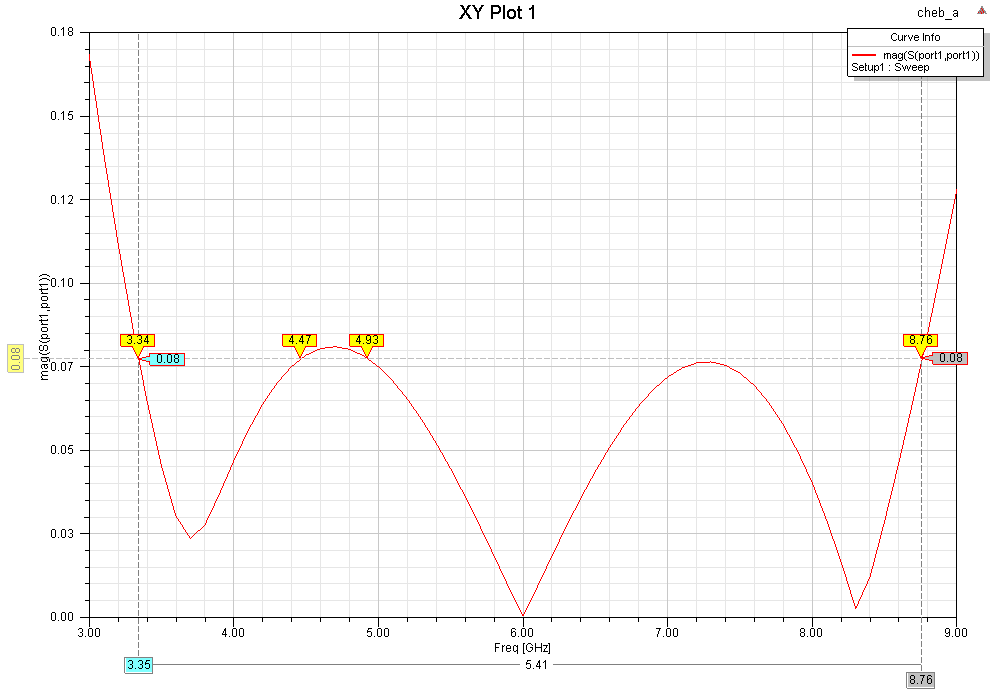
\includegraphics[width=\textwidth]{var_diel_s11_optimized.png}}
  \caption{$\text{S}_{11}$ plot using a Chebyshev transformer with 3 sections with varying dielectric.}
  \label{fig:var_diel_s11}
\end{figure}

\subsection{Part B}\label{sec:1b}
Another way to create a section of the transformer is to vary the height of the sections and use the same dielectric as that of the waveguide. the height of the sections can be calculated from (\ref{eq:height})
\begin{equation}
  b_i=b_0\frac{Z_i}{Z_0}
  \label{eq:height}
\end{equation}
The value of the section height and section length, assuming the waveguide has $\epsilon_r=1$, can be found in Table~\ref{tab:height}
\begin{table}
  \centering
  \caption{Chebyshev transformer properties using variable height.}
  \begin{tabular}{|c|c|c|}\hline
     & $b$ & $\frac{\lambda_g}{4}$ \\ \hline
    $Z_0$ & $\SI{10.00}{\milli\metre}$ & $\SI{13.50}{\milli\metre}$ \\ \hline
    $Z_1$ & $\SI{7.89}{\milli\metre}$ & $\SI{13.50}{\milli\metre}$ \\ \hline
    $Z_2$ & $\SI{5.42}{\milli\metre}$ & $\SI{13.50}{\milli\metre}$ \\ \hline
    $Z_3$ & $\SI{3.73}{\milli\metre}$ & $\SI{13.50}{\milli\metre}$ \\ \hline
    $Z_4$ & $\SI{2.94}{\milli\metre}$ & $\SI{13.50}{\milli\metre}$ \\ \hline
  \end{tabular}
  \label{tab:height}
\end{table}
The simulation results shown in Figure~\ref{fig:var_dim_s11} shows that the theoretical bandwidth ($\Delta f=\SI{6}{\giga\hertz}$) was not achieved with this setup, but instead only $\SI{4.80}{\giga\hertz}$ was achieved. One reason for this could be that the transformer in \textit{HFSS} is not ideal.

\begin{figure}
  \centering
  \noindent\makebox[\textwidth]{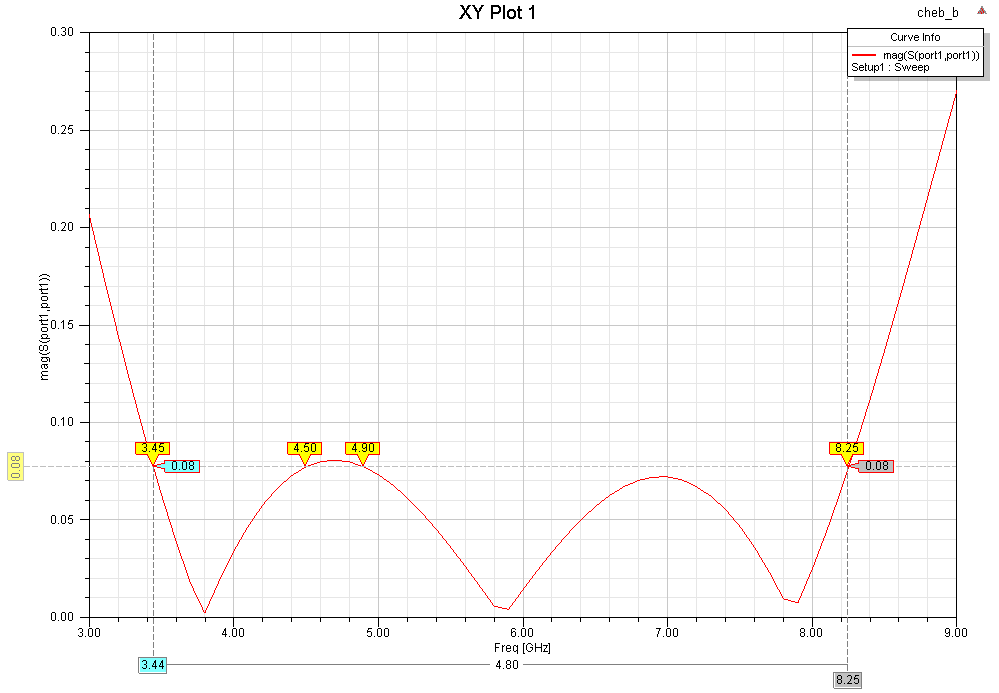
\includegraphics[width=\textwidth]{var_dim_s11_optimized.png}}
  \caption{$\text{S}_{11}$ plot using a Chebyshev transformer with 3 sections with varying height.}
  \label{fig:var_dim_s11}
\end{figure}

\section{Discussion}
The transformer in Section~\ref{sec:1a} has better bandwidth than the transformer in Section~\ref{sec:1b} so theoretically a transformer with variable dielectric should be preferred. In reality it might not be as easy to find materials with dielectric that completely match the desired permittivity while the dimensions of the transformer is much easier to modify so for practical reasons the transformer in Section~\ref{sec:1b} should be preferred.
\end{document}